% =============================================================
% main.tex -- Bachelor Thesis skeleton
% Vietnamese-German University, Faculty of Engineering, CS Program
%
% HOW TO COMPILE (see README.md for details):
%   pdflatex main.tex
%   bibtex main
%   pdflatex main.tex
%   pdflatex main.tex
% =============================================================
\documentclass[12pt]{report}

% ---------- Page geometry (single-spaced, numbered pages by default) ----------
\usepackage[a4paper,margin=1in]{geometry}
\usepackage[utf8]{inputenc}
\usepackage[T1]{fontenc}
\usepackage{times}          % swap for another 12pt-friendly font if your dept prefers
\usepackage{microtype}
\usepackage{indentfirst}    % indent the first line of every paragraph, including after a heading

% ---------- Figures, tables, listings ----------
\usepackage{graphicx}
\usepackage{booktabs}
\usepackage{array}          % >{\centering\arraybackslash}p{} column type for wrapping table headers
\usepackage{caption}
\usepackage{subcaption}
\usepackage{listings}
\usepackage{xcolor}
\usepackage{enumitem}
\usepackage{amsmath}
\usepackage{longtable}      % for the appendix 18-row results table spanning pages
\usepackage{pifont}         % \ding{51}/\ding{55} checkmarks/crosses used in the positioning table
\usepackage{tikz}           % for the conflict-example diagram (fig:conflict-example)
\usetikzlibrary{positioning, arrows.meta}
\usepackage{pdfpages}       % \includepdf for the official cover page (cover.pdf)

% ---------- Cross-references ----------
\usepackage{hyperref}
\hypersetup{
  colorlinks=true,
  linkcolor=black,
  citecolor=black,
  urlcolor=blue,
  pdftitle={AI-Assisted Master Prompt Generation. Challenges and Proposed Solutions.},
}
\usepackage[capitalise,noabbrev]{cleveref}
% cleveref does not know the `listings` package's lstlisting counter/name by
% default; needed for \cref{lst:governance} (App. B.1) to print "Listing N"
% instead of falling back to a bare number.
\crefname{lstlisting}{listing}{listings}
\Crefname{lstlisting}{Listing}{Listings}

% ---------- Bibliography (natbib + bibtex) ----------
% Using classic bibtex instead of biblatex+biber: biber is noticeably
% heavier to invoke and is a common cause of "compile timed out" on
% Overleaf's free plan for even modest documents. natbib+bibtex is lighter
% and sufficient for this document's citation style.
% Author-year (not numbered): the prose throughout this thesis is written
% assuming \citet renders as "Author (Year)" (e.g. "Mondal et al. (2024)
% characterize..."), so the citation style must match -- see \bibliographystyle
% below, which must be an author-year-compatible .bst (not unsrtnat).
\usepackage[authoryear,round]{natbib}

% ---------- Code listing style ----------
\lstdefinestyle{mystyle}{
  basicstyle=\ttfamily\footnotesize,
  keywordstyle=\color{blue}\bfseries,
  commentstyle=\color{gray}\itshape,
  stringstyle=\color{purple!70!black},
  numbers=none,
  breaklines=true,
  breakatwhitespace=true,
  breakindent=0pt,
  xleftmargin=0pt,
  frame=single,
  rulecolor=\color{black!30},
  showstringspaces=false,
  tabsize=2,
  captionpos=b,
}
\lstset{style=mystyle}

\title{AI-Assisted Master Prompt Generation. Challenges and Proposed Solutions.}
\author{Nguyen Thanh Tu}
\date{2026}

\begin{document}

% ================= COVER PAGE (VGU format) =================
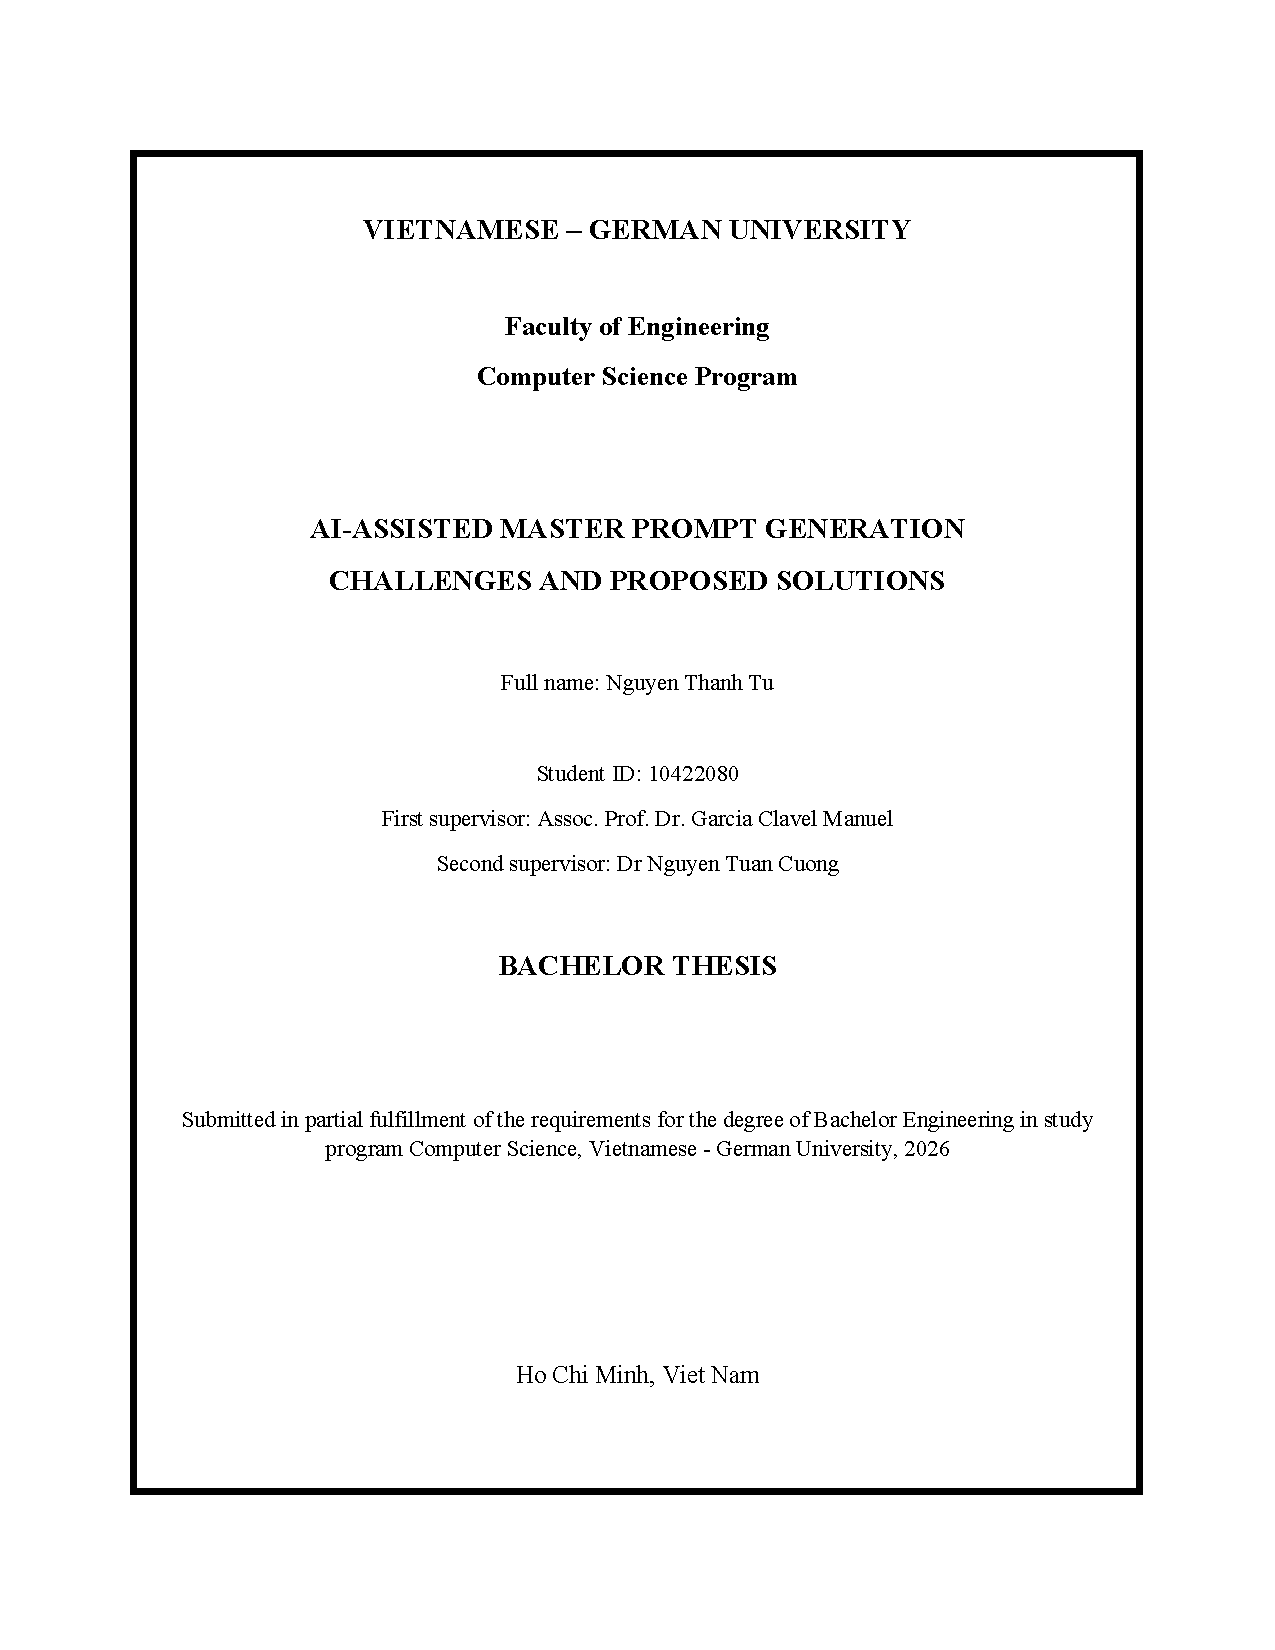
\includepdf[pages=-]{cover.pdf}

% ================= DECLARATION =================
% Declaration page, matching the required VGU thesis declaration format.
\thispagestyle{empty}
\begin{center}
\vspace*{1.5cm}
{\bfseries\Large Declaration}

\vspace{1.2cm}
\end{center}

\noindent
I, Nguyen Thanh Tu, hereby confirm that this thesis is my original work,
completed following registration for the Bachelor of Engineering in
Computer Science degree at Vietnamese -- German University, under the
guidance and supervision of Assoc. Prof. Dr. Garcia Clavel Manuel and
Dr. Nguyen Tuan Cuong. This thesis does not contain material previously
included in a thesis or dissertation submitted to this or any other
institution for a degree, diploma, or other qualification.

\vspace{3cm}

\begin{center}
Signature

\vspace{2cm}

\rule{6cm}{0.4pt}\\[4pt]
Nguyen Thanh Tu\\
Student in the Computer Science Program\\
Faculty of Engineering\\
Vietnamese -- German University
\end{center}

\clearpage


% ================= FRONT MATTER =================
\pagenumbering{roman}
\tableofcontents
\clearpage
\phantomsection
\addcontentsline{toc}{chapter}{List of Tables and Figures}
\chapter*{List of Tables and Figures}
\section*{Tables}
\makeatletter
\@starttoc{lot}
\makeatother
\section*{Figures}
\makeatletter
\@starttoc{lof}
\makeatother
\clearpage
\pagenumbering{arabic}

% ================= CHAPTERS =================
\chapter{Introduction}
\label{chap:introduction}

\section{Motivation}
\label{sec:motivation}

When developers work with AI coding agents, the requirements of a project are
rarely expressed in a single instruction. Instead, the developer's intent
evolves across a long and unstructured prompt history containing initial
requests, follow-up questions, corrections, removals, replacements, and changes
of direction. Although this history records how the project developed, it does
not provide a clear description of what the project should be in its current
state. Earlier requirements may no longer apply, later prompts may replace
previous values, and some messages may concern temporary implementation
decisions rather than the intended product.

To make the project easier to continue or transfer, developers can create a
\emph{master prompt}. In this thesis, a master prompt is a single,
self-contained specification of the user's currently valid intent. It should
describe what must be built without requiring another developer or AI agent to
read the entire prompt history. It should keep active requirements, reflect
later changes, and leave out requirements that were removed or replaced.

Recently, AI coding agents can build much of a software project from a clear set
of prompts. This makes the prompts used to describe the project an important
part of the project itself. Work on spec-driven development also shows that a
written specification can be kept and used to guide the generated code
\citep{piskala2026specdriven}. In the same way, a master prompt can be treated
as a useful project artifact rather than a temporary summary. It can be saved,
updated, and kept together with the code so that the project can be continued
in another AI session, by another coding agent, or by another developer.

However, creating a faithful master prompt is not only a summarization task.
The agent must separate what the user actually requested from details that
appeared during implementation. In practical coding, an AI agent may add architectural
patterns, filenames, technologies, validation rules, or other choices that the
user never asked for. This problem is closely related to \emph{extrinsic hallucination}, which
\citet{ji2023survey} describe as generated content that is not supported by
the source. In master-prompt consolidation, these unsupported additions may
make the result appear more complete while reducing its faithfulness to the
user's original requests.

The main concern is therefore not only whether an AI agent can produce a
clear and compact document, but whether every requirement in that document is
traceable to the prompt history. A faithful master prompt should preserve all
currently valid requirements, correctly reflect removals and replacements, and
exclude both agent-added details and outdated requirements. Although carefully
written consolidation instructions may improve the result, it remains unclear
how strongly instruction strictness affects traceability and whether stricter
prompting continues to improve the result for longer and more realistic
development histories.

A second challenge arises when the master prompt is treated not only as the
output of a one-time consolidation process, but as a persistent project
artifact. After handoff, a later session or another contributor may introduce a
new instruction that contradicts a requirement already established in the
master prompt. Such contradictions may use different wording that may unintentionally
modify, replace, or even remove already existing requirements without recognizing the contradiction.
Moreover, they may appear in different parts of the master prompt rather than next to each
other. They are therefore semantic conflicts rather than text-level merge conflicts.
If the agent silently chooses one value, combines incompatible requirements,
or overwrites the existing requirement, the master prompt can no longer serve
as a reliable representation of the project's intent.

Together, these problems motivate a spec-guided approach that keeps the current requirements
and their sources explicit, and checks each new instruction against the
existing specification before updating it.

\section{Problem Statement}
\label{sec:problem-statement}

This thesis studies two connected problems in AI-assisted master prompt
construction:

\begin{itemize}[leftmargin=*]
\item \textbf{Non-traceable consolidation.}
This problem occurs when an agent consolidates the full prompt history. The
resulting master prompt may contain details that the user never requested,
such as technologies, filenames, design choices, or added rules. It may also
retain old requirements after they were removed, undone, or replaced. At the
same time, some valid requirements may be omitted. These errors make the
master prompt less faithful even when its wording is clear and its overall
meaning appears similar to the original history.

\item \textbf{Semantic conflict in a persistent master prompt.}
This problem occurs when a new prompt is added after the master prompt has
already been created. The new instruction may contradict an existing
requirement, but the agent may fail to report the conflict. Instead, it may
silently overwrite the old value, combine two incompatible values, or keep
both requirements in different parts of the document. In each case, the
master prompt no longer provides one consistent description of the project.
\end{itemize}

To address these problems, this thesis evaluates several single-pass
consolidation instructions and proposes a \emph{spec-guided} approach. Rather
than consolidating the raw prompt history only at the end of a session, the
proposed approach maintains an explicit specification of the current user
intent under a governance instruction. Each new prompt is checked against the
existing requirements before the specification is updated. Potential conflicts
are surfaced together with their source requirements instead of being silently
resolved.

\section{Research Questions}
\label{sec:research-questions}

\begin{description}[leftmargin=*,style=nextline]
\item[RQ1]
To what extent do AI-generated master prompts contain non-traceable content,
including agent-added requirements and outdated requirements that should
have been removed or replaced? How does consolidation instruction strictness
(\emph{basic}, \emph{loose}, and \emph{strict}) affect this problem?

\item[RQ2]
Does a spec-guided consolidation approach produce a more traceable master
prompt than single-pass consolidation of the raw prompt history using basic,
loose, or strict instructions?

\item[RQ3]
When a later instruction semantically conflicts with a settled requirement,
how can a spec-guided approach surface the conflict, trace it to both
requirements, and avoid resolving it without user input?
\end{description}

\section{Contributions}
\label{sec:contributions}

This thesis makes the following contributions:

\begin{itemize}[leftmargin=*]

\item A requirement-level evaluation method for master-prompt traceability.
Instead of comparing whole documents, the method splits each master prompt
into atomic requirements and uses entailment-based scoring with AlignScore
\citep{zha2023alignscore} to determine whether each requirement is supported
by the human-consolidated ground truth. Paired examples are also used to show
why word similarity alone is not a reliable measure of traceability. Applied
to 24 master-prompt candidates produced by three agents, four consolidation
approaches, and two projects, the method answers RQ1 by showing that stricter
single-pass instructions reduce non-traceable content, but the improvement
stops before reaching the ground truth
(\cref{chap:experiment-traceability}).

\item A consolidation method called \texttt{spec\_guided}, which maintains a
living specification under an explicit governance instruction. Instead of
rebuilding the master prompt from the full prompt history only at the end of
the session, the method checks each new prompt and updates the specification
throughout the session. This method answers RQ2. Compared with each agent's
own single-pass baseline, it improves traceability in four of the six
agent--project pairs. Manual analysis of the other two pairs identifies
trade-offs caused by making requirement decisions repeatedly during the
session rather than once at the end
(\cref{chap:experiment-traceability}).

\item A project-handoff method for identifying semantic conflicts in a settled
master prompt. The method uses a separate governance instruction that checks
each later prompt against the existing specification, preserves settled
requirements when the intended change is unclear, and records both conflicting
requirements for the user to resolve. The method is demonstrated using five
constructed conflicts and two compatible controls across the simple and hard
projects (\cref{chap:experiment-conflict}).

\end{itemize}

\chapter{Related Work}
\label{chap:related-work}

Among the studies on AI-assisted development, several studies
are relevant to the problems addressed in this thesis. This chapter
reviews work on prompt consolidation and project handoff, errors in consolidated
requirements, requirement traceability evaluation, methods for keeping
specifications up to date, and semantic conflict detection. The final section
brings these areas together and identifies the research gap addressed by this
thesis.

\section{Prompt Consolidation and Project Handoff}
\label{sec:related-consolidating}

The work most directly related to prompt consolidation is presented by
\citet{mondal2024consolidating}. The study shows how users solve an issue through
sequences of prompts and propose combining those prompts into a single prompt.
Their main goal is to reduce repeated interaction and produce the desired
answer more efficiently. They do not study about whether every statement in the
consolidated prompt can be traced to the original prompt sequence. They also
do not examine how later prompts remove, undo, or replace earlier
requirements.

Recent work has also studied how an AI coding task can be continued after a
handoff. \citet{kc2026handoffdebt} describe \emph{handoff debt}: the work a
new coding agent must repeat to understand an interrupted task. Their focus is
on transferring repository state and task information so that another agent
can resume the work. This differs from the present thesis, which studies how
faithfully the current project intent can be represented in one master
prompt.

Another approach is to preserve the interaction history rather than
consolidate it. \citet{santoni2026cmv} propose a graph-based memory system that
keeps previous interaction turns available for later retrieval. This avoids
reducing the full history to one document. The present research studies a
different case: the history is deliberately turned into a single portable
artifact that can be read, stored, and handed over.

\section{Errors in Consolidated Requirements}
\label{sec:related-loss}

The main failure studied in this thesis is that a generated master prompt may
contain requirements that are not supported by the user's prompt history.
This can be understood through existing work on hallucination.

\citet{ji2023survey} distinguish between intrinsic and extrinsic
hallucination. Intrinsic hallucination occurs when generated content
contradicts its source. Extrinsic hallucination occurs when generated content
cannot be supported by the source. This, by definition, is relevant to master-prompt
consolidation. A technology, filename, validation rule, or design choice that
the user never requested is unsupported requirements and is therefore close to
extrinsic hallucination. 

A different error occurs when the master prompt retains an old requirement
after a later prompt has changed, removed, or replaced it. This content
originally appeared in the prompt history, so it is not unsupported in the
same way as extrinsic hallucination. Instead, it reflects a failure to 
follow the order of user's prompts and recover the user's current intent.

Related work has also used language models to obtain software requirements
from conversations. \citet{voria2025recover} propose RECOVER, which finds
and generates system requirements from stakeholder conversations. This shows
that unstructured dialogue can be used as a source of requirements. However,
RECOVER focuses on generating requirements from stakeholder discussions. Unlike 
the problem addressed by \citet{voria2025recover}, the prompt history already
contains direct development instructions, but their current state must be 
recovered after modifications, removals, replacements, and changes of direction.

\section{Evaluating Requirement Traceability}
\label{sec:related-metrics}

Word similarity alone is not reliable enough for evaluating a master prompt. Two
requirements may use almost the same words while conflicting with each other in meaning.
In contrast, two requirements can use different words while expressing the same
requirement. For this reason, this study uses entailment-based evaluation to check whether the meaning of a candidate requirement is supported by the ground truth.

\citet{zha2023alignscore} propose AlignScore, a factual-consistency metric that
measures whether a claim is supported by a context. The model treats the two
inputs differently: one is the source context and the other is the claim being
checked. In this thesis, the manually constructed ground truth is used as the
context and each candidate requirement is used as the claim:

\[
\mathrm{ALIGN}
(\mathrm{context}=\mathrm{ground\ truth},\
\mathrm{claim}=\mathrm{candidate\ requirement}).
\]

A low score means that the candidate requirement is not well supported by the
ground truth. This makes AlignScore suitable for finding agent-added details
and outdated requirements.

The evaluation is performed at the requirement level rather than on the full
master prompt. This choice is related to FActScore and Claimify.
\citet{min2023factscore} evaluate long-form text by first separating it into
atomic facts and then checking whether each fact is supported.
\citet{metropolitansky2025claimify} study how complex text can be separated
into clear and independent claims. This thesis uses the same
general idea but treats each unit as an atomic software requirement.

This requirement-level evaluation gives each requirement its own score, making it
possible to identify exactly which parts of a master prompt are unsupported.
It also prevents well-supported requirements from hiding a small number of
incorrect ones. The scores from individual requirements
can then be used to calculate the untraceable rate and to support 
human review of the errors found in each candidate.

Traceability has also been studied between other software artifacts.
\citet{alor2025traceability} evaluate whether language models can create trace
links between software documentation and source code. Their artifacts and
evaluation setting are different from those in this thesis, but there is 
common concern about whether one artifact is supported by another.
However, in this thesis, each generated requirement is checked against
the ground-truth master prompt to determine whether 
it is supported by the user's original requirements.

\section{Keeping an Up-to-Date Specification}
\label{sec:related-spec}

Spec-driven development provides a related view of how natural language
requirements can be used during AI-assisted development. \citet{piskala2026specdriven} describe approaches in which a specification is
kept as the main description of what the software should do, while code is
generated or checked against it.

The \texttt{spec\_guided} method in this thesis uses a similar principle.
Instead of asking an agent to rebuild the current requirements from the full
prompt history only at the end, it keeps a specification updated throughout
the session. The specification records the requirements that are currently
valid, while the original prompts are kept separately as their source.

This thesis does not treat the specification as a complete replacement for
code, nor does it claim to implement a full spec-driven development system.
It uses the maintained-specification idea for a narrower purpose: reducing
non-traceable content during master-prompt construction and giving the agent
a current document against which later instructions can be checked.

Prompts can also become maintained artifacts in software projects.
\citet{tafreshipour2025wild} study how prompts stored in software repositories
change over time and report inconsistencies between prompt revisions. Their
work examines repository-based prompts rather than the developer--agent prompt
histories studied in this thesis. However, it supports the view that prompts
may need to be stored and maintained carefully when they remain part of a
project over time.

\section{Semantic Conflict Detection}
\label{sec:related-vc}

A text document can merge successfully while still containing requirements
that conflict in meaning. Such a conflict is called a semantic conflict.
Related work in collaborative code generation shows the same difference 
between text-level consistency and semantic correctness.

\citet{pugachev2025codecrdt} propose CodeCRDT, which allows multiple coding
agents to edit shared code while avoiding text-level merge conflicts.
Their preliminary inspection suggests that 5--10\% of the inspected runs
still contain semantic problems such as duplicate declarations and type
mismatches. This result is not a complete measurement of semantic-conflict
frequency, but it shows an important point: a clean text-level merge
does not guarantee a correct result.

CodeCRDT studies conflicts in source code. Unlike source code, it cannot be checked by a compiler, type checker, or test suite, and there is no exact score that can always determine whether two requirements conflict. The conflict must therefore be identified by comparing their meanings. Thus, this thesis shows that the conflict must be found 
by comparing the meaning of the incoming instruction with the meaning of 
the existing specification.

The work most closely related to the conflict part of this thesis is
\emph{Semantic Commit} by \citet{vaithilingam2025semanticcommit}. Their system
helps users add new information to an existing intent specification, such as a
Cursor rules file or game design document. It uses a knowledge graph and
retrieval to find existing information that may be affected by the update.
The retrieved information is then classified as a direct conflict, an
ambiguous conflict, or a non-conflict. The interface presents the result to
the user and supports human review and resolution.

Semantic Commit also evaluates a baseline called DropAllDocs, which provides
the complete existing information store to the model instead of retrieving
selected parts. The present thesis uses a related full-context idea because
the tested master prompts are small enough to fit in the model context.
However, it does not reproduce Semantic Commit's knowledge-graph retrieval
pipeline or its user interface.

The main difference is the starting point. Semantic Commit assumes that an
intent specification already exists and studies how new information should be
added to it. This thesis first studies whether such a specification can be
constructed faithfully from a long prompt history. It then reuses the
maintained specification to check next instructions for conflict. In other
words, Semantic Commit mainly addresses updates to an existing intent
specification. It does not study how that specification was created from
the earlier development history, while RQ1 and RQ2 examine how a traceable master prompt is
created before updating the specification.

The decision not to resolve a conflict automatically is also related to the
intent gap described by \citet{lahiri2026intent}. A model may produce an
implementation that appears reasonable while still differing from what the
user intended. When two requirements cannot both be true and the user's
preferred value is not clear, silently selecting one value may create the
same problem. The safer action is to report the conflict and ask the user to
decide.

\section{Research Gap}
\label{sec:positioning}

The reviewed work can be compared along three parts of the problem: producing
one consolidated artifact, checking whether its content is supported by the
source prompts, and reporting semantic conflicts when the artifact is updated.

Prompt consolidation by \citet{mondal2024consolidating} addresses the first
part, but its purpose is interaction efficiency rather than requirement
traceability. AlignScore \citep{zha2023alignscore}, FActScore
\citep{min2023factscore}, and Claimify \citep{metropolitansky2025claimify}
provide useful ideas for evaluating support at a fine level, but they do not
construct or maintain a master prompt. Spec-driven development
\citep{piskala2026specdriven} supports the use of a maintained specification,
but does not directly evaluate whether an AI-generated master prompt contains
requirements that the user never requested. CodeCRDT
\citep{pugachev2025codecrdt} shows that text-level convergence does not
prevent semantic errors, but it works on source code rather than
natural-language requirements.

Semantic Commit \citep{vaithilingam2025semanticcommit} is the closest work for
conflict detection because it checks new information against an existing
intent artifact and keeps the user involved in resolution. However, it begins
with an intent specification that has already been prepared. It does not
study whether consolidating a raw, ordered prompt history introduces
unsupported requirements or retains values that were later changed.

Among the works reviewed in this chapter, the specific combination studied in
this thesis remains open: evaluating the traceability of a master prompt built
from a chronological AI coding history, comparing single-pass consolidation
with a maintained-specification method, and testing whether the same method
can report later semantic conflicts without silently resolving them.

\chapter{Methodology}
\label{chap:methodology}

This chapter describes the two experiments conducted in this thesis. It first
summarizes their design (\cref{sec:method-overview}), then presents the
datasets and ground truths used in Experiment~1 (\cref{sec:method-dataset}),
the consolidation pipeline used in Experiment~1 (\cref{sec:method-pipeline}), and the
traceability evaluation used for RQ1 and RQ2
(\cref{sec:method-metrics}). Finally, the full design of Experiment~2, which
addresses semantic conflict handling in RQ3, is presented separately in
\cref{chap:experiment-conflict}.

\section{Overview of the Experiments}
\label{sec:method-overview}

This thesis contains two experiments:

\begin{itemize}[leftmargin=*]
  \item \textbf{Experiment~1: Traceability Evaluation (RQ1 and RQ2).}
  This experiment uses two project histories, three AI coding agents, and four
  consolidation strategies. RQ1 compares the three single-pass strategies:
  \emph{basic}, \emph{loose}, and \emph{strict}. RQ2 evaluates the proposed
  \emph{spec-guided} strategy against these baselines. Together, the four
  strategies produce 24 master-prompt candidates, which are evaluated using
  mean AlignScore and untraceable rate.
  \item \textbf{Experiment~2: Semantic Conflict Handling (RQ3).}
  This experiment begins with the hand-built ground-truth master prompt of each
  project as a settled specification. The simple project receives one
  conflicting instruction and one compatible control, while the hard project
  receives four conflicting instructions and one compatible control. Claude,
  Codex, and Gemini are tested under three conditions:
  \emph{consolidate-then-ask}, \emph{do-not-resolve}, and
  \emph{spec-guided}. The experiment examines how each condition represents
  semantic conflicts without automatically selecting between incompatible
  requirements.
\end{itemize}

The following sections describe the dataset, consolidation pipeline, and
traceability evaluation used in Experiment~1. The complete design and evaluation criteria
of Experiment~2 are presented in
\cref{chap:experiment-conflict}.

\section{Dataset and Ground Truth}
\label{sec:method-dataset}

Two synthetic project histories were created for controlled evaluation,
summarized in \cref{tab:dataset-overview}. They are different in length, complexity,
and writing style.

\begin{table}[htbp]
  \centering
  \caption{Overview of the two evaluation projects.}
  \label{tab:dataset-overview}
  \begin{tabular}{@{}llp{9.7cm}@{}}
    \toprule
    Project & Prompts & Description \\
    \midrule
    simple project & 12 & A small portal project with navigation
      requirements, a conditional color rule, a contact form, and several
      later navigation changes. \\
    hard project & 45 & A larger ERP-style application with customers,
      vendors, products, orders, invoices, reports, roles, and permissions.
      Its history contains more revisions, removals, and conversational
      wording. \\
    \bottomrule
  \end{tabular}
\end{table}

A ground-truth master prompt was constructed manually for each project. The
prompts were read in their original order, and only the requirements that
remained valid at the end of the history were retained. A later modification
replaced the earlier value, while a removal or undo instruction deleted the
affected requirement when no replacement was given. Details that did not
originate from the user's prompts were excluded.

The ground truth was also split manually into atomic requirements. Then, when the
LLM split the candidate master prompts, these ground-truth requirements
were used to check whether a candidate unit combined too many requirements or
split one requirement into unnecessarily small parts.

Every Experiment~1 candidate is evaluated against the ground truth for the
same project. Both ground-truth master prompts are also used as settled
starting artifacts in Experiment~2. The simple-project case introduces one
conflict and one compatible control, while the hard-project case introduces
four conflicts and one compatible control.

\section{Consolidation Pipeline}
\label{sec:method-pipeline}

Each project history was replayed with three AI coding agents:

\begin{itemize}[leftmargin=*]
  \item Claude, using Claude Sonnet 4.6;
  \item Codex, using GPT-5.5-Codex;
  \item Gemini, using Gemini Flash 3.5.
\end{itemize}

Separate sessions were used for each agent, project, and strategy. The project
prompts were delivered in their original order.

Before Prompt~1, every session received the same fixed setup message
(\cref{sec:pre-experiment}). It instructed the agent to treat all next
requests as part of one project and to remain in the same workspace. It also
stated that the setup message was not a software requirement and must not
appear in the master prompt.

\subsection{Consolidation Strategies}

Experiment~1 compares four strategies, summarized in
\cref{tab:consolidation-variants}.

\begin{table}[htbp]
  \centering
  \caption{The four consolidation strategies used in Experiment~1.}
  \label{tab:consolidation-variants}
  \begin{tabular}{@{}lp{9.5cm}@{}}
    \toprule
    Strategy & Description \\
    \midrule
    \texttt{basic\_prompt} & The agent is asked to consolidate the ordered
      prompt history into one master prompt. No explicit traceability rule is
      provided. \\
    \texttt{loose\_consolidate} & The basic instruction is extended by asking
      the agent to reflect later modifications and removals and to avoid
      additional or missing features. \\
    \texttt{strict\_consolidate} & The loose instruction is extended with an
      explicit traceability rule: every requirement must originate from the
      numbered prompts, and unrequested or non-traceable details must be excluded. \\
    \texttt{spec\_guided} & The agent records the raw prompts in
      \texttt{prompts.md} and maintains the current master prompt in
      \texttt{spec.md} after every new instruction. \\
    \bottomrule
  \end{tabular}
\end{table}

The first three strategies are single-pass approaches. The agent receives the
complete history and creates the master prompt once, at the end. Their
instructions are cumulative: \texttt{loose\_consolidate} adds a faithfulness
clause to \texttt{basic\_prompt}, and \texttt{strict\_consolidate} adds an
explicit traceability rule. The exact templates are reproduced in
\cref{app:consolidation-prompts}.

The fourth strategy, \texttt{spec\_guided}, maintains the master prompt
throughout the session under a standing governance instruction. It uses two
files:

\begin{itemize}[leftmargin=*]
  \item \texttt{prompts.md}, an append-only, verbatim log of the numbered
  project prompts;
  \item \texttt{spec.md}, the current master prompt containing only the
  requirements that remain valid.
\end{itemize}

After each new prompt, the agent records it in \texttt{prompts.md} and updates
\texttt{spec.md}. Compatible requirements are added, while clear
modifications, replacements, removals, and undo instructions update the
affected topic immediately.

When a prompt changes an existing topic, the agent reconstructs that topic
from its relevant prompt history instead of editing the current sentence
locally. This helps remove outdated values and conversation-dependent wording.
The development of this rule is described in
\cref{sec:rq2-governance}.

If a new instruction cannot hold together with a settled requirement and does
not clearly indicate a deliberate revision, the agent leaves the current
specification unchanged and records the conflict for the user to decide. The
same conflict-handling principle is applied in Experiment~2 through a
separate governance instruction written for the project-handoff setting.

At the end of the session, \texttt{spec.md} itself is used as the candidate
master prompt. The full governance instruction is reproduced in
\cref{lst:governance}.

This method borrows the general spec-driven development principle that the
specification can act as the main statement of what should be built
\citep{piskala2026specdriven}. It does not implement a complete spec-driven
development toolchain; \texttt{spec.md} is used here only to maintain a
traceable master prompt.

\section{Traceability Metrics}
\label{sec:method-metrics}

Experiment~1 evaluates whether the requirements stated in each candidate are
supported by the ground truth. The evaluation focuses on content that appears
in the candidate but is not part of the final user intent, including
agent-added details and outdated requirements.

\subsection{Atomic Requirement Decomposition}

A whole-document score can hide a small number of unsupported requirements
among many correct ones. Each candidate is therefore evaluated one atomic
requirement at a time.

The decomposition follows the general idea of Claimify
\citep{metropolitansky2025claimify}, but this thesis does not run the Claimify
system. Instead, a fixed prompt designed for software requirements is applied
to each candidate sentence using an LLM
(\cref{sec:decomp-prompt}).

The prompt uses a keep-all approach. It retains unsupported details,
outdated requirements, conversational statements, and any other content in
the candidate so that these units remain available for scoring.

The ground truth and candidates are decomposed differently:

\begin{itemize}[leftmargin=*]
  \item the ground-truth atomic requirements are created manually during
  ground-truth construction;
  \item candidate requirements are first generated by the fixed LLM
  decomposition prompt.
\end{itemize}

The candidate requirements were first split by an LLM using the fixed
decomposition prompt. The LLM did not receive the complete ground-truth master
prompt or its list of atomic requirements for the candidate.
However, the few-shot examples in the prompt followed the same splitting
decisions used when creating the ground truth.

After the LLM produced the candidate requirements, the author compared them
with the manually split ground truth to check that both were divided at a
similar level of detail. If one candidate unit combined two or more requirements 
that were separate in the ground truth, it was divided into smaller units. 
If the LLM split one requirement into unnecessarily small parts, those parts were kept
together. This review changed only how the candidate text was divided; it did
not remove, rewrite, or correct its content.

The ground truth itself was split manually because the decomposition prompt
sometimes divided one enumeration into several weaker requirements. For
example, a requirement defining four navigation buttons could become four
separate requirements, losing the meaning that the four buttons together form
one complete set.

Both the ground-truth construction and the candidate-decomposition review were
performed by the same author. The possible influence of this process on the
evaluation is discussed in \cref{sec:discussion-limitations}.


\subsection{AlignScore}

AlignScore measures whether a candidate requirement is supported by the
ground truth \citep{zha2023alignscore}:

\[
\mathrm{ALIGN}(\text{context}, \text{claim}) \rightarrow [0,1].
\]

For each atomic candidate requirement $r$, the complete ground-truth master
prompt is used as the context:

\[
\mathrm{AlignScore}(r) = \mathrm{ALIGN}(\text{context}=\text{ground truth},\ \text{claim}=r).
\]

The scores are computed in \texttt{nli\_sp} mode using the AlignScore-large
checkpoint with a RoBERTa-large backbone. The comparison in
\cref{sec:demo-experiment} explains why entailment is used instead of word or
embedding similarity.

Two values are reported for each candidate:

\begin{itemize}[leftmargin=*]
  \item \textbf{Mean AlignScore}: the average score across its atomic
  requirements;
  \item \textbf{Untraceable rate}: the percentage of requirements with an
  AlignScore below $0.5$.
\end{itemize}

The untraceable rate indicates how many candidate requirements are not strongly
supported by the ground truth and therefore require further inspection. A
requirement below the threshold is treated as potentially untraceable, not
automatically as invented. As shown in \cref{sec:rq2-results}, some faithful
short requirements also receive unexpectedly low scores.

This is a precision-style evaluation because it checks only the content
included in the candidate. It does not measure whether the candidate omitted
a valid ground-truth requirement. Ground-truth coverage is therefore left as
a limitation (\cref{sec:discussion-limitations}).



\chapter{Experiment 1: Traceability Evaluation (RQ1, RQ2)}
\label{chap:experiment-traceability}

This chapter reports the traceability evaluation for RQ1 and RQ2. It first
explains why semantic support is more suitable than word similarity for this
task. It then compares the three single-pass strategies and evaluates the
proposed \emph{spec-guided} strategy. Finally, it examines the low-scoring
requirements to clarify what the automatic results actually represent.

Experiment~1 uses two project histories and three AI coding agents. For each
agent and project, four master-prompt construction strategies are evaluated:
\emph{basic}, \emph{loose}, \emph{strict}, and \emph{spec-guided}. The first
three strategies produce the eighteen single-pass candidates used to answer
RQ1. The six \emph{spec-guided} candidates are used to answer RQ2, giving 24
candidates in total. Each candidate is evaluated at the atomic-requirement
level using mean AlignScore and untraceable rate. The complete experimental
procedure is described in \cref{chap:methodology}, while the exact project
histories and instructions are reproduced in \cref{app:datasets}.

\section{Why Word Similarity Is Not Enough}
\label{sec:demo-experiment}

A faithful master prompt must preserve the meaning of the original
requirements. Similar wording alone is not sufficient because changing one
value, condition, or permission can reverse the meaning of a requirement.

Before AlignScore was selected, it was compared with BERTScore precision
\citep{zhang2020bertscore} on two sentence pairs. The first pair contains
almost identical wording but opposite meanings. The second is a faithful
paraphrase taken from a real candidate.

\begin{lstlisting}[breaklines=true, basicstyle=\small\ttfamily, caption={Two sentence pairs scored with BERTScore precision and AlignScore.}, label={lst:demo-pairs}]
Pair 1 -- contradiction
Ground truth: "A navigation label starting with H must have a blue background."
Candidate:    "A navigation label starting with H must have a red background."
BERTScore (P) = 0.98        AlignScore = 0.0002

Pair 2 -- faithful paraphrase
Ground truth: "Implement customer management with create, edit, delete, and browse operations."
Candidate:    "Include customer management: Users can create, edit, delete, and browse customers."
BERTScore (P) = 0.63        AlignScore = 0.87
\end{lstlisting}

In Pair~1, only the color changes, but this makes the candidate contradict the
ground truth. BERTScore still gives it $0.98$ because most of the wording is
unchanged. AlignScore instead checks whether the candidate is supported by the
ground truth, so the score falls to $0.0002$.

Pair~2 expresses the same customer-management requirement with different
wording. BERTScore gives it only $0.63$, while AlignScore recognizes the
semantic support and gives it $0.87$.

These examples show why an entailment-based metric is used in this thesis.
Traceability requires distinguishing a contradiction from a faithful
paraphrase, not only measuring how similar two sentences appear.

\section{Results on the Single-Pass Strategies}
\label{sec:results-18}

RQ1 compares three single-pass strategies: \emph{basic}, \emph{loose}, and
\emph{strict}. Each strategy was tested with three agents on two projects,
producing eighteen master-prompt candidates.

Each candidate was divided into atomic requirements using the procedure
described in \cref{sec:method-metrics}. Every candidate requirement was then
scored against the complete ground-truth master prompt for the same project.

Two values are reported:

\begin{itemize}[leftmargin=*]
  \item \textbf{Mean AlignScore}: the average score across all requirements
  in the candidate;
  \item \textbf{Untraceable rate}: the percentage of requirements with an
  AlignScore below $0.5$.
\end{itemize}

A requirement below $0.5$ is treated as requiring further inspection. It is
not automatically considered non-traceable because some faithful requirements also
receive unexpectedly low scores.

\begin{table}[htbp]
  \centering
  \caption{Requirement-level AlignScore results for the simple project, reported as mean AlignScore (untraceable rate).}
  \label{tab:results-simple}
  \begin{tabular}{@{}lcccc@{}}
    \toprule
    Agent & \emph{basic} & \emph{loose} & \emph{strict} & \emph{spec-guided} \\
    \midrule
    Claude & 0.086 (92\%) & 0.824 (10\%) & 0.988 (0\%) & 0.989 (0\%) \\
    Codex  & 0.387 (62\%) & 0.857 (18\%) & 0.828 (18\%) & 0.987 (0\%) \\
    Gemini & 0.083 (97\%) & 0.737 (21\%) & 0.917 (10\%) & 0.989 (0\%) \\
    \bottomrule
  \end{tabular}
\end{table}

\begin{table}[htbp]
  \centering
  \caption{Requirement-level AlignScore results for the hard project, reported as mean AlignScore (untraceable rate).}
  \label{tab:results-hard}
  \begin{tabular}{@{}lcccc@{}}
    \toprule
    Agent & \emph{basic} & \emph{loose} & \emph{strict} & \emph{spec-guided} \\
    \midrule
    Claude & 0.382 (62\%) & 0.362 (67\%) & 0.905 (3\%) & 0.882 (11\%) \\
    Codex  & 0.787 (19\%) & 0.772 (21\%) & 0.860 (10\%) & 0.895 (8\%) \\
    Gemini & 0.391 (68\%) & 0.414 (60\%) & 0.865 (10\%) & 0.785 (17\%) \\
    \bottomrule
  \end{tabular}
\end{table}

The clearest difference is between \emph{basic} and \emph{strict}. The
\emph{strict} strategy achieves a higher mean AlignScore and a lower
untraceable rate for all six agent--project pairs. For example, Claude rises
from $0.086$ to $0.988$ on the simple project, while Gemini rises from
$0.391$ to $0.865$ on the hard project.

The improvement is not steady from \emph{basic} to \emph{loose} to
\emph{strict} in every case. On the hard project, \emph{loose} performs
slightly worse than \emph{basic} for Claude and Codex. On the simple project,
Codex has a slightly higher mean score with \emph{loose} than with
\emph{strict}, while both have the same untraceable rate.

Nevertheless, \emph{strict} outperforms \emph{loose} in five of the six
comparisons. The results therefore support the use of an explicit
traceability rule. They do not support the broader claim that adding more
instructions always leads to steady improvement.

These scores evaluate only the requirements included in a candidate. They do
not show whether the candidate omitted a valid ground-truth requirement.
Ground-truth coverage is therefore not measured in this experiment.

\section{The Spec-Guided Strategy}
\label{sec:rq2-design}

The three RQ1 strategies create the master prompt once, after the complete
prompt history has been provided. RQ2 examines whether traceability improves
when the master prompt is maintained throughout the session.

The proposed \emph{spec-guided} strategy maintains two files:

\begin{itemize}[leftmargin=*]
  \item \texttt{prompts.md}, an append-only record of the original prompts;
  \item \texttt{spec.md}, the current master prompt containing the
  requirements that remain valid.
\end{itemize}

After each new prompt, the instruction is recorded and \texttt{spec.md} is
updated. Compatible requirements are added. Clear modifications, removals,
and undo instructions update the affected topic. If a new instruction
conflicts with a settled requirement without clearly revising it, the conflict
is reported rather than silently resolved.

The complete procedure is described in \cref{sec:method-pipeline}, and the
governance instruction is reproduced in \cref{lst:governance}. During its
development, two recurring problems were found.

\section{Developing the Governance Instruction}
\label{sec:rq2-governance}

Both problems came from the same behavior: the agents tended to edit the
existing sentence using the latest prompt's wording instead of writing a
complete requirement from the relevant prompt history.

\subsection{Failure Mode 1: Edit Instructions Remain in the Specification}
\label{sec:rq2-edit-wording}

Some prompts describe how an earlier requirement should change rather than
directly stating the final requirement. For example:

\begin{quote}
  \emph{Use top navigation instead.}
\end{quote}

and:

\begin{quote}
  \emph{Change navigation buttons: Dashboard, Policies, History, Contact.}
\end{quote}

These instructions are clear in the original conversation because the earlier
state is still available. In a standalone master prompt, however, ``instead''
refers to information that may no longer be present, while ``Change
navigation buttons'' describes an edit rather than the final requirement. 

Early versions of the governance preserved this wording in
\texttt{spec.md}. Simply removing individual words such as ``instead'' or ``change''
was not a reliable solution. For example, deleting ``Change'' left
the requirement without a verb.

The final rule therefore works at the topic level. When a new prompt affects
an existing topic, the agent must read the relevant prompts and write one new
sentence stating the current requirement. It must not patch the previous
sentence with the latest wording.

For example:

\begin{quote}
  \emph{Change navigation buttons: Dashboard, Policies, History, Contact.}
\end{quote}

becomes:

\begin{quote}
  \emph{Add 4 navigation buttons: Dashboard, Policies, History, Contact.}
\end{quote}

This rule also applies to changed names, values, counts, and conditions.

\subsection{Failure Mode 2: Conversational Wording Remains in the Specification}
\label{sec:rq2-conversational-wording}

The hard project contains more conversational wording. For example:

\begin{quote}
  \emph{I'd like to build a simple ERP web application for a small business.
  Let's start with a clean foundation that we can gradually expand.}
\end{quote}

The actual requirements are to build the application and give it a clean,
expandable foundation. Expressions such as ``I'd like to'' and ``Let's start
with'' belong to the conversation rather than to the final specification.

Similar cases include temporary comments or reasons for requesting a feature,
such as:

\begin{quote}
  \emph{The dashboard doesn't need much yet.}
\end{quote}

and:

\begin{quote}
  \emph{Since we're buying from suppliers, let's add vendor management too.}
\end{quote}

These expressions originate from real prompts, but not all of their wording
describes what the system must implement.

The same topic-level rule also addresses this problem. The agent keeps the
requested names, values, conditions, and constraints, but writes them as a
standalone requirement.

For example:

\begin{quote}
  \emph{Build a simple ERP web application for a small business with a clean
  foundation that can be gradually expanded.}
\end{quote}

The two failure modes therefore share one solution: reconstruct the current
requirement from the relevant prompt history instead of preserving the latest
prompt as a local sentence edit.

\begin{lstlisting}[breaklines=true, basicstyle=\small\ttfamily, caption={Examples observed while developing the spec-guided governance instruction.}, label={lst:rq2-governance-examples}]
simple project

Navigation buttons
Before: "Change navigation buttons: Dashboard, Policies, History, Contact."
After:  "Add 4 navigation buttons: Dashboard, Policies, History, Contact."

Navigation layout
Before: "Use top navigation instead."
After:  "Use top navigation."

hard project

Project introduction
Before: "I'd like to build a simple ERP web application for a small business. Let's start with a clean foundation that we can gradually expand."
After:  "Build a simple ERP web application for a small business with a clean foundation that can be gradually expanded."
\end{lstlisting}

\section{RQ2 Results}
\label{sec:rq2-results}

The \emph{spec-guided} strategy performs better than the same agent's
\emph{strict} result in four of the six comparisons.

\begin{table}[htbp]
  \centering
  \caption{\emph{Spec-guided} compared with the same agent's \emph{strict} result. Bold marks the better result in each row.}
  \label{tab:rq2-vs-strict}
  \begin{tabular}{@{}llcc@{}}
    \toprule
    Project & Agent & \emph{strict} & \emph{spec-guided} \\
    \midrule
    simple project & Claude & 0.988 (0\%)  & \textbf{0.989} (\textbf{0\%})  \\
    simple project & Codex  & 0.828 (18\%) & \textbf{0.987} (\textbf{0\%}) \\
    simple project & Gemini & 0.917 (10\%) & \textbf{0.989} (\textbf{0\%})  \\
    hard project   & Claude & \textbf{0.905} (\textbf{3\%})  & 0.882 (11\%)  \\
    hard project   & Codex  & 0.860 (10\%) & \textbf{0.895} (\textbf{8\%})  \\
    hard project   & Gemini & \textbf{0.865} (\textbf{10\%}) & 0.785 (17\%) \\
    \bottomrule
  \end{tabular}
\end{table}

On the simple project, all three \emph{spec-guided} candidates reach a
$0\%$ untraceable rate. The final outputs also avoid the edit-oriented
navigation wording found during development.

On the hard project, only Codex improves on its \emph{strict} result. Its mean
AlignScore rises from $0.860$ to $0.895$, while its untraceable rate falls
from $10\%$ to $8\%$. Claude and Gemini both receive lower automatic
scores with \emph{spec-guided}.

However, the low-scoring requirements do not all represent invented content.
Manual review identified three different causes.

\subsection{Review of Low-Scoring Requirements}

\textbf{Same requirements with inconsistent wording.}
Some low-scoring candidate requirements describe the same system behavior as
the ground truth but use shorter or less consistent requirement wording. For
example:

\begin{quote}
\emph{Introduce user roles: Admin, Staff, and Manager}
\end{quote}

receives an AlignScore of $0.265$ against:

\begin{quote}
\emph{Support the user roles Admin, Manager, and Staff.}
\end{quote}

Similarly, \emph{Add sales orders} receives a score of $0.274$ against
\emph{Implement sales orders}. In both cases, the candidate preserves the
intended feature, but uses a different requirement verb from the ground truth.

These examples show that, although the governance is designed to keep the
output close to the original prompts, it does not always produce consistent
software-requirement wording. The agents may use verbs such as ``Add'' or
``Introduce'' where the ground truth uses ``Implement'' or ``Support.''
AlignScore also has difficulty recognizing that these sentences express the
same software requirement despite their different wording. The same low
scores were obtained when the sentence pairs were evaluated separately,
showing that the results were repeatable rather than caused by the other
requirements in the candidate.

\textbf{Non-requirement content.}
Some low-scoring text comes directly from the prompts but expresses a reason,
transition, or temporary comment rather than a requirement that must remain in
the master prompt.

For example, the request for an Excel export explains that the file should be
shared with an accountant. The export feature is a requirement, while the
accountant clause is the reason for requesting it.

Expressions such as \emph{The dashboard doesn't need much yet} create the
same problem. They are not invented, but they do not state a complete
requirement.

\textbf{Hallucinated details.}
Gemini's hard-project candidate contains two clear additions that do not
appear in the original prompts:

\begin{itemize}[leftmargin=*]
  \item an Admin-only User Accounts management view;
  \item Vendors added to a navigation bar that was requested to contain only
  Dashboard, Customers, and Products.
\end{itemize}

These details are hallucinations as they introduce system behavior or
interface elements that cannot be traced to the original prompt history. They
show that repeatedly applying the no-invention rule reduces, but does not
completely prevent, hallucinated content from entering the maintained
specification.

\subsection{Interpretation}

The manual review shows that the automatic results should not be read as a
direct count of hallucinated requirements. The requirements below the $0.5$
threshold fall into the three categories described above: same requirements
with inconsistent wording, non-requirement content, and hallucinated
details.

Codex shows the clearest improvement on the hard project. Its mean AlignScore
increases from $0.860$ to $0.895$, while its untraceable rate decreases from
$10\%$ to $8\%$. Most of its low-scoring units either describe the same
system behavior as the ground truth but use different requirement wording, or
contain incomplete conversational expressions. The manual review did not find
comparable hallucinated functionality in these units. The automatic and manual
results therefore both indicate an improvement over its \emph{strict}
baseline.

Claude's untraceable rate increases from $3\%$ to $11\%$, but this does not
mean that $11\%$ of its requirements are hallucinations. Several flagged
requirements describe the same system behavior as the ground truth but use
shorter or different verbs, such as ``Add'' instead of ``Implement'' or
``Introduce'' instead of ``Support.'' Although the governance is designed to
keep the output close to the original prompts, it does not always produce
consistent software-requirement wording. AlignScore also has difficulty
recognizing that these sentences express the same software requirement
despite their different wording. Claude additionally retains some unnecessary
conversational wording, but no hallucinated feature was found during the
manual review. Its result is therefore closer to the \emph{strict} baseline
than the raw untraceable rate suggests.

Gemini shows a different result. Some of its flagged requirements also use
inconsistent wording or preserve conversational material, but its candidate
contains two hallucinated details: an Admin-only User Accounts management view
and Vendors added to the navigation bar. Its lower score therefore reflects a
real decrease in traceability. However, the $17\%$ untraceable rate should not
be interpreted as the percentage of hallucinated requirements because only
part of that rate comes from the two hallucinations.

The untraceable rate is therefore most useful as a screening measure. It shows
which requirements require manual inspection, but it does not identify the
cause of each low score. A flagged unit may express the same requirement with
inconsistent wording, retain text from the conversation that is not a final
requirement, or introduce content that was never requested.

Overall, the \emph{spec-guided} strategy improves on \emph{strict} in four
of the six agent--project comparisons. It performs strongly for all three
agents on the shorter simple project, but its results are mixed on the longer
hard project: Codex improves, Claude remains close to its baseline after
manual review, and Gemini introduces two hallucinated details.

RQ2 therefore does not show that per-turn consolidation is always more
traceable than a single final consolidation. Maintaining \texttt{spec.md}
reduces the amount of history that must be reconstructed in one step, but
every update requires the agent to interpret the new prompt and rewrite the
affected requirement correctly. As the history becomes longer, these repeated
updates create more opportunities for inconsistent wording, unnecessary
conversational text, or hallucinated details to enter the specification. This
trade-off is discussed further in \cref{sec:discussion-tradeoff}.


\chapter{Experiment 2: Semantic Conflict in a Master Prompt (RQ3)}
\label{chap:experiment-conflict}

A master prompt can become a shared project artifact that is passed to a later
session or contributor. In this setting, a new instruction may conflict with a
requirement already settled in the artifact.

Experiment~2 uses the settled master prompts of both projects to examine this
problem. It compares three conflict-handling conditions, including a separate
\emph{spec-guided} governance instruction written for the project-handoff
setting. This instruction follows the same general conflict-handling principle
as the RQ2 method, but it is a different prompt.

\section{Defining a Semantic Conflict}
\label{sec:conflict-setting}

A \emph{semantic conflict} occurs when two requirements cannot both hold. For
example, a settled master prompt may state:

\begin{quote}
\emph{Invoices should have a due date 15 days after they are created.}
\end{quote}

A later prompt may then request:

\begin{quote}
\emph{Add a reminder that gets sent 3 days before an invoice's 30-day due
date.}
\end{quote}

The later prompt does not directly ask to change the due date, but it assumes
a 30-day value that conflicts with the settled 15-day requirement. This
differs from a clear revision such as:

\begin{quote}
\emph{Change the invoice due date to 30 days.}
\end{quote}

A clear revision explicitly replaces the earlier value. A semantic conflict
instead occurs when a later prompt assumes or introduces an incompatible value
without clearly stating that the settled requirement should be changed.

The model cannot reliably determine whether the user intended a revision or
simply overlooked the earlier requirement \citep{lahiri2026intent}. Silently
selecting either value may therefore change the user's intent
\citep{liu2025condorcet}.

Semantic conflicts may be difficult to notice because the requirements can use
different wording and appear in separate parts of the master prompt. Unlike
line-based tools such as \texttt{git}, which detect overlapping text changes,
they require comparing requirements by meaning
\citep{pugachev2025codecrdt}.

\section{Experimental Design}
\label{sec:conflict-data}

Experiment~2 uses the hand-built ground-truth master prompts of both projects
as settled project artifacts. Every run follows the same sequence: the agent
receives a fixed handoff prompt, the settled master prompt \(M\) for the
selected project, and then the later prompts one at a time.

\subsection{Handoff and Starting Master Prompts}

After the pre-experiment setup, the same neutral handoff prompt is used in
every condition:

\begin{quote}
\emph{Here is the consolidated result of the earlier prompts for this project.
Continue the project from here. I will then send more prompts, one at a time.}
\end{quote}

The corresponding ground-truth master prompt is then provided as \(M\). The
hard-project \(M\) represents the settled result of its 45-prompt history,
while the simple-project \(M\) represents the settled result of its 12-prompt
history.

Using the ground truths ensures that all agents begin with the same correct
project state. The experiment can therefore focus on conflict handling rather
than errors introduced during earlier consolidation.

\subsection{Later Prompts}

The hard-project case contains four conflict prompts and one compatible
positive control. The simple-project case contains one conflict prompt and one
compatible positive control. All prompts are sent one at a time.

The conflicts are written as ordinary feature requests that assume something
incompatible with \(M\), without clearly asking to replace the settled
requirement. The five conflicts are summarized in
\cref{tab:conflict-taxonomy}, and their exact wording is reproduced in
\cref{app:conflict-prompts}.

\begin{table}[htbp]
  \centering
  \caption{The five semantic conflicts used in Experiment~2.}
  \label{tab:conflict-taxonomy}
  \small
  \begin{tabular}{@{}llp{4.5cm}p{4.5cm}@{}}
    \toprule
    Project & Type & Settled in \(M\) & Assumed by the later prompt \\
    \midrule
    Hard & Value & The invoice due date is 15 days. & A reminder is sent three days before an invoice's 30-day due date. \\
    Hard & Scope & Only vendors use the recycle bin; customers are permanently deleted. & The customers page has a recycle-bin tab and a Restore button. \\
    Hard & Layout & The application uses a top navigation bar. & A button collapses and expands a left sidebar. \\
    Hard & Permission & Staff cannot delete products. & An audit entry records when a staff member deletes their own product. \\
    Simple & Value & The navigation contains four buttons. & All five navigation buttons wrap onto two rows on small screens. \\
    \bottomrule
  \end{tabular}
\end{table}

In the simple-project case, \(M\) defines four navigation buttons:
Dashboard, Policies, History, and Contact. The later prompt refers to five
buttons without requesting an additional button, creating a conflict between
the settled and assumed counts.

The print-button prompt in the hard project and the footer prompt in the
simple project serve as positive controls. Neither conflicts with its
corresponding master prompt and both should be added normally.

\Cref{fig:conflict-example} illustrates the hard-project due-date conflict
under the three conditions.

\begin{figure}[htbp]
  \centering
  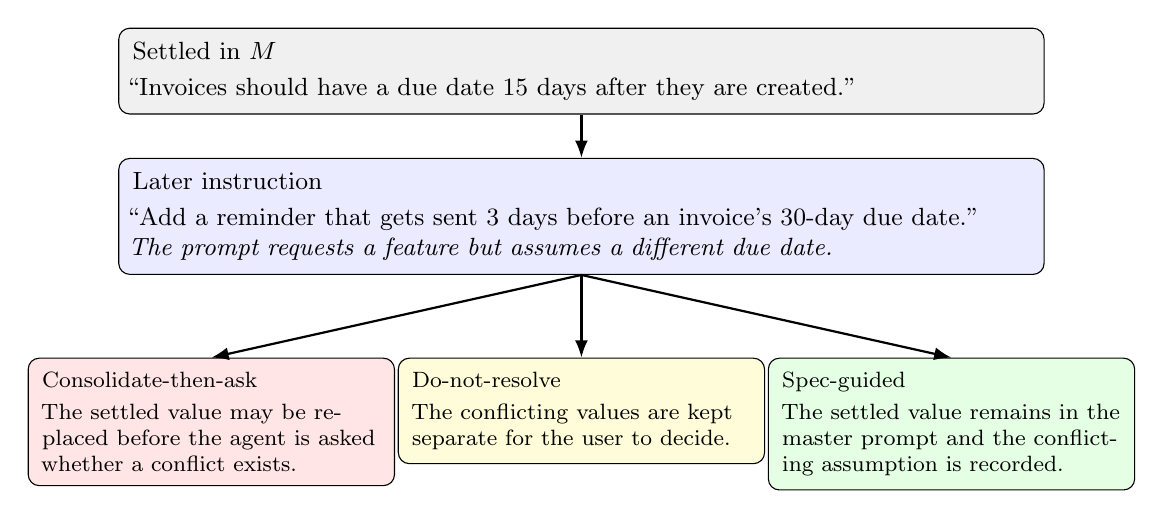
\begin{tikzpicture}[
      box/.style={draw, rounded corners, align=left, inner sep=5pt,
        font=\small},
      settled/.style={box, fill=gray!12, text width=11.4cm},
      newp/.style={box, fill=blue!8, text width=11.4cm},
      cond/.style={box, fill=white, text width=4.3cm,
        font=\footnotesize},
      bad/.style={cond, fill=red!10},
      mid/.style={cond, fill=yellow!15},
      good/.style={cond, fill=green!10},
      lbl/.style={font=\bfseries\small},
      condlbl/.style={font=\bfseries\footnotesize},
      arr/.style={-{Latex[length=2.2mm]}, thick},
    ]

    \node[settled] (m) {
      \lbl{Settled in \(M\)}\\[2pt]
      ``Invoices should have a due date 15 days after they are created.''
    };

    \node[newp, below=0.55cm of m] (p) {
      \lbl{Later instruction}\\[2pt]
      ``Add a reminder that gets sent 3 days before an invoice's 30-day due
      date.''\\
      \emph{The prompt requests a feature but assumes a different due date.}
    };

    \node[bad, below=1.05cm of p, xshift=-4.7cm] (c1) {
      \condlbl{Consolidate-then-ask}\\[2pt]
      The settled value may be replaced before the agent is asked whether a
      conflict exists.
    };

    \node[mid, below=1.05cm of p] (c2) {
      \condlbl{Do-not-resolve}\\[2pt]
      The conflicting values are kept separate for the user to decide.
    };

    \node[good, below=1.05cm of p, xshift=4.7cm] (c3) {
      \condlbl{Spec-guided}\\[2pt]
      The settled value remains in the master prompt and the conflicting
      assumption is recorded.
    };

    \draw[arr] (m) -- (p);
    \draw[arr] (p.south) -- (c1.north);
    \draw[arr] (p.south) -- (c2.north);
    \draw[arr] (p.south) -- (c3.north);
  \end{tikzpicture}

  \caption{The due-date conflict under the three experimental conditions.}
  \label{fig:conflict-example}
\end{figure}

\section{Conflict-Handling Conditions}
\label{sec:conflict-conditions}

Claude, Codex, and Gemini are tested under the three conditions shown in
\cref{tab:conflict-conditions}. For each project, every condition receives the
same setup prompt, handoff prompt, settled master prompt \(M\), and later
prompts. The conditions differ only in how conflicts are handled.

\begin{table}[htbp]
  \centering
  \caption{The three conflict-handling conditions.}
  \label{tab:conflict-conditions}
  \begin{tabular}{@{}lp{9cm}@{}}
    \toprule
    Condition & Procedure \\
    \midrule
    \emph{Consolidate-then-ask} & The agent consolidates \(M\) and the later prompts using the \emph{strict} instruction. It is asked about conflicts only after the new master prompt has been produced. \\
    \emph{Do-not-resolve} & The \emph{strict} instruction is extended with a rule that conflicting values must not be selected or merged. The conflict is listed separately for the user to decide. \\
    \emph{Spec-guided} & The separate Experiment~2 governance instruction is active while the later prompts are processed. Each prompt is checked against the settled master prompt when it arrives. \\
    \bottomrule
  \end{tabular}
\end{table}

The comparison examines whether checking for conflicts only after
consolidation is sufficient, whether a direct no-resolution rule prevents
silent replacement, and whether continuous checking preserves settled
requirements as later prompts arrive.

\section{The Spec-Guided Conflict-Handling Method}
\label{sec:conflict-detector}

The \emph{spec-guided} condition uses the final Experiment~2 governance
instruction reproduced in \cref{lst:conflict-governance}. Unlike the RQ2
governance instruction, which maintains \texttt{prompts.md} and
\texttt{spec.md} from the beginning of a project, this instruction begins
with an already-settled master prompt handed to a new session.

Each later prompt is checked against \(M\). Compatible requirements are added,
while clear revisions update the affected requirement. If a later prompt
cannot coexist with a settled requirement and does not clearly request a
change, the settled requirement remains in the master prompt. Both conflicting
requirements are listed under \texttt{\#\# Unresolved conflicts}, and the user
is asked which one should be kept.

When consolidation is requested, the agent returns the conflict-free
requirements under \texttt{\#\# Master prompt} and any unresolved conflicts
in a separate section. The decision is based on the meaning of the
requirements rather than fixed words such as ``change'' or ``instead.''

Semantic Commit provides a related approach in which new instructions are
checked against requirements retrieved from an intent store
\citep{vaithilingam2025semanticcommit}. Retrieval is not required here because
the complete master prompt fits within the model's context. The governance
instruction therefore checks the settled artifact directly.

\section{Evaluation Criteria}
\label{sec:conflict-evaluation}

Each conflict is manually reviewed using the criteria in
\cref{tab:conflict-evaluation}. The review checks whether the agent detects the
conflict, avoids resolving it automatically, preserves the settled
requirement, introduces no new details, and identifies both source
requirements.

\begin{table}[htbp]
  \centering
  \caption{Manual evaluation criteria for each semantic conflict.}
  \label{tab:conflict-evaluation}
  \small
  \begin{tabular}{@{}lp{9.2cm}@{}}
    \toprule
    Criterion & Expected behavior \\
    \midrule
    Conflict detection & The incompatible requirements are reported as a conflict. \\
    No automatic resolution & The agent does not select or merge the conflicting values without user input. \\
    Preservation & The settled requirement remains in the master prompt. \\
    No invention & No new value, condition, or technical detail is introduced. \\
    Source identification & The settled requirement and the conflicting later prompt are identified. \\
    \bottomrule
  \end{tabular}
\end{table}

The print-button and footer prompts are evaluated separately as positive
controls. They should be added without being reported as conflicts.

The experiment is a qualitative demonstration. The criteria define how the
outputs are inspected, but they are not used to calculate a general
conflict-detection score.

\section{Threats to Validity}
\label{sec:conflict-threats}

Experiment~2 is a small qualitative study based on five constructed conflicts
and two compatible controls. Although the cases cover value, scope, layout,
and permission conflicts, they do not represent every inconsistency that may
occur in real projects. Their direct wording may also make them easier to
detect than longer or more ambiguous conflicts.

Model outputs are non-deterministic, and only a small number of runs were
performed. The observed behavior may therefore vary across repeated sessions.

Finally, the conflicts, expected behavior, and outputs were reviewed by the
same author who designed the experiment. Without an independent rater,
interpretation and evaluation bias cannot be ruled out.

\chapter{Discussion, Limitations, and Future Work}
\label{chap:discussion}

This chapter discusses the main findings from Experiment~1 and the
implications of the conflict-handling method introduced in Experiment~2. The results
show that explicit traceability rules improve master-prompt consolidation.
However, updating the specification after every prompt requires the agent to
make more decisions about how each new instruction should be interpreted,
which can introduce new errors. They also show that traceability alone is not sufficient when the
master prompt is handed to a later session, because new prompts may conflict
with already-settled requirements.

\section{Discussion}

\subsection{Traceability in Single-Pass Consolidation}

The main RQ1 finding is that a direct traceability rule is more effective than
a general request to preserve the meaning of the prompt history. The
\emph{strict} strategy performs better than \emph{basic} in all six
agent--project comparisons and better than \emph{loose} in five of them
(\cref{sec:results-18}).

However, the results do not show that adding more instructions always improves
the output. The \emph{loose} strategy occasionally performs worse than
\emph{basic}, while Codex performs slightly better with \emph{loose} than
with \emph{strict} on the simple project. Therefore, what matters is not the
length of the consolidation prompt, but whether it clearly limits the output
to requirements found in the original history.

Even the \emph{strict} strategy does not remove all non-traceable content.
This suggests that prompting can reduce unsupported additions, but cannot
guarantee a fully traceable master prompt.

\subsection{The Trade-Off in Spec-Guided Consolidation}
\label{sec:discussion-tradeoff}

The \emph{spec-guided} strategy improves on \emph{strict} in four of the six
agent--project comparisons. It performs well for all three agents on the
simple project, but only Codex improves on the hard project
(\cref{sec:rq2-results,tab:rq2-vs-strict}).

Maintaining the specification after every prompt reduces the need to
reconstruct the full project history at the end. However, it also requires the
agent to make a decision on every turn: whether the new prompt adds, changes,
removes, or conflicts with an existing requirement.

This becomes difficult when prompts contain conversational wording or several
changes to the same topic. Text that explains why a feature is requested may
be copied into the specification even though it is not itself a requirement.
Likewise, an instruction such as ``Change navigation buttons'' must be
rewritten as the resulting requirement rather than preserved as an editing
command.

The simple project contains short and direct prompts, so these interpretation
risks are limited. The hard project contains longer revision chains and more
conversational language, creating more opportunities for small errors to enter
the maintained specification.

The \emph{spec-guided} strategy should therefore be understood as an
alternative workflow, not as a guaranteed improvement over single-pass
consolidation. It reduces one large reconstruction problem, but replaces it
with many smaller interpretation decisions.

\subsection{Interpreting the Evaluation Scores}

The requirement-level evaluation helps identify which parts of a candidate
need inspection, but a low AlignScore does not always mean that the model
invented a requirement.

The manual review identified three main causes of low scores: the same
requirement expressed with different wording, conversational content that does
not belong in the final specification, and genuinely hallucinated details.
The untraceable rate combines these cases and should therefore be treated as a
screening measure rather than a direct hallucination rate.

The evaluation also measures only whether the requirements included in a
candidate are supported by the ground truth. It does not measure whether valid
requirements were omitted. A high score can therefore indicate strong
traceability without proving that the master prompt is complete.

\subsection{Semantic Conflicts After Project Handoff}

RQ3 considers how later prompts are handled after a settled master prompt is
handed to a new session. A requirement may conflict with an earlier decision
even when the two use different wording and do not create a direct text-level
clash.

The Experiment~2 governance instruction checks each later prompt against the
settled master prompt. Compatible additions are accepted, clear revisions
update the affected requirement, and unclear conflicts are listed under
\texttt{\#\# Unresolved conflicts} for the user to decide.

The method is demonstrated on both project histories using five constructed
conflicts and two compatible controls. Its purpose is to prevent an unclear
conflict from being silently treated as a project decision while allowing
compatible work to continue.

\section{Limitations and Threats to Validity}
\label{sec:discussion-limitations}

\begin{itemize}[leftmargin=*]

\item \textbf{Limited dataset.}
The evaluation uses two author-created web application histories, five
constructed semantic conflicts, and two compatible controls. The findings may
not generalize to larger projects, other domains, or different prompt-writing
styles.

\item \textbf{Limited repeated runs.}
Experiment~1 uses one scored candidate for each condition, while
Experiment~2 remains a small qualitative study. Because model outputs are
non-deterministic, some observed differences may not represent stable
behavior.

\item \textbf{Single-author evaluation.}
The ground truth, requirement decomposition review, and conflict labels were
produced by the same author. Without an independent reviewer, interpretation
and evaluation bias cannot be ruled out.

\item \textbf{Metric coverage.}
AlignScore is sensitive to wording and requirement decomposition. The
evaluation also does not measure requirements that are missing from the
candidate master prompt.

\end{itemize}

\section{Future Work}
\label{sec:discussion-future}

\begin{itemize}[leftmargin=*]

\item Repeat the evaluation with more runs and more realistic project
histories.

\item Add an evaluation of missing requirements and use more independent
reviewers for ground truth and manual labels.

\item Test the handoff method with more conflicts, compatible additions, and
clear revision prompts.

\item Evaluate whether the governance rules are more effective when the master
prompt is updated after each prompt or when the complete history is
consolidated only once at the end of the session.


\end{itemize}

\chapter{Conclusion}
\label{chap:conclusion}

This thesis studied how AI agents consolidate a sequence of project prompts
into a master prompt while preserving the user's original requirements. The
main concern is that a generated master prompt may appear clear and complete
while containing details that were never requested, retaining requirements
that were later removed, or silently replacing a settled requirement with an
incompatible one.

The traceability experiment showed that the consolidation instruction has a
clear effect on the result. A general request to summarize or preserve meaning
does not always prevent non-traceable content. The \emph{strict} strategy,
which explicitly requires every requirement to come from the original prompt
history, performs better than \emph{basic} in all tested agent--project
comparisons and better than \emph{loose} in most comparisons. However, 
even this direct rule does not eliminate all non-traceable content.

The \emph{spec-guided} strategy explored a different approach by maintaining
the master prompt throughout the original project session. This reduces the
need to reconstruct the complete history at the end, but the results show a
trade-off. The method improves four of the six comparisons with
\emph{strict}, including all three agents on the simple project, but performs
worse for two agents on the hard project. Maintaining the specification on
every turn introduces repeated decisions about whether a prompt adds, changes,
removes, or conflicts with an existing requirement. These decisions become
more difficult in long and conversational prompt histories.

The requirement-level AlignScore evaluation helps identify candidate
requirements that may need inspection. However, the manual review shows that a
low score does not always represent invented content. It may also result from
different wording or from conversational text that was preserved even though
it is not a final requirement. The metric is therefore useful for comparing
candidates and locating possible problems, but it should be used together with
manual review. It also does not measure requirements that were omitted from
the candidate.

Experiment~2 treats the master prompt as a shared project artifact handed to a
new session. It uses both project histories to demonstrate how later prompts
can conflict with settled requirements without directly requesting that the
earlier decisions be changed.

The proposed governance instruction checks each later prompt against the
settled master prompt. Compatible additions are accepted, clear revisions
update the existing requirement, and unclear conflicts are kept separate for
the user to resolve. The method does not attempt to select the correct value
automatically; its purpose is to prevent the agent from silently turning an
ambiguous instruction into a project decision.

Overall, the findings show that a master prompt should not be treated as a
simple summary generated at the end of a coding session. It is a project
specification derived from a sequence of user decisions. Its requirements
should remain traceable to the original prompts, and later changes should be
checked against what has already been settled.

No single prompting strategy completely removes interpretation errors.
Single-pass consolidation must reconstruct the final state from the full
history, while per-turn consolidation introduces many smaller decisions that
can fail independently. A reliable workflow therefore requires both explicit
traceability rules and human review of unclear changes or conflicts.

The practical implication is that teams using a master prompt as a shared
artifact should maintain it carefully rather than regenerate it as an
uncontrolled summary. Keeping the original prompt history, updating the
current specification as decisions change, and asking the user to resolve
unclear conflicts can better preserve intent across AI-assisted development
sessions.


% ================= REFERENCES =================
\bibliographystyle{plainnat}
\bibliography{references}

% ================= APPENDIX =================
% Per the formatting rules: statistics, matrices, illustrations belong here
% and are NOT counted in the 25-60 page body scope.
\appendix
\chapter{Full Traceability Results}
\label{app:results}

This appendix reports the complete results of Experiment~1 for the simple and
hard projects, extending the per-project tables in
\cref{tab:results-simple,tab:results-hard}. The experiment compares three
single-pass consolidation strategies---\emph{basic}, \emph{loose}, and
\emph{strict}---with the \emph{spec-guided} strategy across Claude, Codex,
and Gemini.

For each candidate, \cref{tab:full-results-appendix} reports the number of
atomic requirements (\emph{Units}), the mean AlignScore, and the percentage of
requirements with an AlignScore below $0.5$ (\emph{Untraceable rate}). The
evaluation method is described in \cref{sec:method-metrics}, while the main
results are discussed in \cref{sec:results-18,sec:rq2-results}.

\begin{longtable}{@{}llccc@{}}
  \caption{Complete requirement-level traceability results for
  Experiment~1.}
  \label{tab:full-results-appendix} \\
  \toprule
  Project & Candidate & Units & Mean AlignScore & Untraceable rate \\
  \midrule
  \endfirsthead
  \multicolumn{5}{c}{\tablename\ \thetable{} -- continued} \\
  \toprule
  Project & Candidate & Units & Mean AlignScore & Untraceable rate \\
  \midrule
  \endhead
  \midrule \multicolumn{5}{r}{Continued on next page} \\
  \endfoot
  \bottomrule
  \endlastfoot
  simple project & Claude \emph{basic}        & 12 & 0.086 & 92\% \\
  simple project & Claude \emph{loose}        & 10 & 0.824 & 10\% \\
  simple project & Claude \emph{strict}       & 10 & 0.988 &  0\% \\
  simple project & Claude \emph{spec-guided}  & 10 & 0.989 &  0\% \\
  simple project & Codex \emph{basic}         & 16 & 0.387 & 62\% \\
  simple project & Codex \emph{loose}         & 11 & 0.857 & 18\% \\
  simple project & Codex \emph{strict}        & 11 & 0.828 & 18\% \\
  simple project & Codex \emph{spec-guided}   & 10 & 0.987 &  0\% \\
  simple project & Gemini \emph{basic}        & 36 & 0.083 & 97\% \\
  simple project & Gemini \emph{loose}        & 14 & 0.737 & 21\% \\
  simple project & Gemini \emph{strict}       & 10 & 0.917 & 10\% \\
  simple project & Gemini \emph{spec-guided}  & 10 & 0.989 &  0\% \\
  \midrule
  hard project & Claude \emph{basic}          & 77 & 0.382 & 62\% \\
  hard project & Claude \emph{loose}          & 75 & 0.362 & 67\% \\
  hard project & Claude \emph{strict}         & 29 & 0.905 &  3\% \\
  hard project & Claude \emph{spec-guided}    & 46 & 0.882 & 11\% \\
  hard project & Codex \emph{basic}           & 78 & 0.787 & 19\% \\
  hard project & Codex \emph{loose}           & 82 & 0.772 & 21\% \\
  hard project & Codex \emph{strict}          & 73 & 0.860 & 10\% \\
  hard project & Codex \emph{spec-guided}     & 52 & 0.895 &  8\% \\
  hard project & Gemini \emph{basic}          & 57 & 0.391 & 68\% \\
  hard project & Gemini \emph{loose}          & 48 & 0.414 & 60\% \\
  hard project & Gemini \emph{strict}         & 29 & 0.865 & 10\% \\
  hard project & Gemini \emph{spec-guided}    & 52 & 0.785 & 17\% \\
\end{longtable}

For the single-pass strategies, \emph{strict} performs better than
\emph{basic} in all six agent--project comparisons and better than
\emph{loose} in five. The only exception is Codex on the simple project,
where \emph{loose} has a slightly higher mean AlignScore, while both
strategies have the same untraceable rate.

The \emph{spec-guided} strategy improves on \emph{strict} in four of the six
comparisons. It produces the strongest results for all three agents on the
simple project and improves the Codex result on the hard project. For Claude
and Gemini on the hard project, however, \emph{strict} performs better.

These results show that an explicit traceability rule consistently improves
single-pass consolidation. Maintaining the master prompt throughout the
session can improve the result further, but its effectiveness depends on the
complexity of the project history and the agent being used.

\chapter{Datasets and Experimental Prompts}
\label{app:datasets}

This appendix provides the exact inputs used in the experiments. It contains
the common session-setup prompt, the consolidation instructions used in
Experiment~1, the Experiment~1 \texttt{spec\_guided} governance instruction,
the requirement-decomposition prompt, both project histories, the common
handoff prompt and later instructions used in Experiment~2, and the separate
governance instruction used by its \emph{spec-guided} condition.

All prompts inside the listings are reproduced verbatim. The project
histories are the inputs from which the candidates were produced and the
ground-truth master prompts were manually constructed
(\cref{sec:method-dataset}).

\section{Pre-Experiment Session Setup}
\label{sec:pre-experiment}

Before the first numbered project prompt, every session received the same
setup message. This applies to all 24 candidates in Experiment~1 and every run
in Experiment~2.

The message serves two purposes. First, it keeps all later instructions within
one project and one workspace. Second, it states explicitly that the setup
message is not a software requirement. It is therefore excluded from the
ground truth and candidate master prompts by design, rather than being removed
later during consolidation.

The setup message is not counted as Prompt~1. Numbering begins with the first
actual project instruction.

\begin{lstlisting}[breaklines=true, basicstyle=\small\ttfamily, caption={Pre-experiment setup prompt, sent once before Prompt 1 of every session.}, label={lst:pre-experiment}]
The following instructions are only for setting up our conversation. They are not part of the software project's requirements and must not be included if you are later asked to summarize, consolidate, or generate a master prompt for the project.

Throughout this conversation, treat every subsequent request as part of the same software project. Only work within the current project folder and do not create a new project or switch to another workspace unless I explicitly ask you to.

Acknowledge these instructions and wait for the first project prompt.
\end{lstlisting}

Experiment~2 uses the same setup message before the handoff sequence. The
fixed handoff prompt is then sent, followed by the settled master prompt $M$
for the selected project and its later instructions. The setup message is
administrative and is kept separate from the requirements against which the
later prompts are checked.

\section{Single-Pass Consolidation Prompts}
\label{app:consolidation-prompts}

The three single-pass strategies use cumulative instructions.
\texttt{basic\_prompt} provides the base instruction.
\texttt{loose\_consolidate} adds the second clause to the base instruction.
\texttt{strict\_consolidate} uses the base instruction, the loose clause, and
the final traceability rule together.

\begin{lstlisting}[breaklines=true, basicstyle=\small\ttfamily, caption={\texttt{basic\_prompt}: base consolidation instruction.}]
I have given you a sequence of prompts to build a project, in order. Some prompts added a new requirement, some changed an earlier requirement, and some canceled or undo an earlier requirement completely. Read them in the exact order given. Create a master prompt that consolidate all of them into one single prompt.
\end{lstlisting}

\begin{lstlisting}[breaklines=true, basicstyle=\small\ttfamily, caption={Additional clause used by \texttt{loose\_consolidate}.}]
Make sure that if I have modified or remove a requirement, this is correctly reflected in the final single prompt. The final single prompt should have the exact same meaning of all prompts without any additional or missing features.
\end{lstlisting}

\begin{lstlisting}[breaklines=true, basicstyle=\small\ttfamily, caption={Additional traceability rule used by \texttt{strict\_consolidate}.}]
Important rule: every requirement in the master prompt must be something I actually wrote in one of these prompts. Do not add any requirement, detail, file name, library, or design choice that I did not explicitly ask for, even if it seems like a reasonable or natural thing to include. If something is not directly traceable back to one of these numbered prompts, leave it out.
\end{lstlisting}

\section{Spec-Guided Governance Instruction for Experiment 1}
\label{sec:governance-instruction}

The fourth strategy in Experiment~1 does not create the master prompt through
a final single-pass request. Instead, it maintains a living specification
throughout the original project session.

The governance instruction below was placed in the agent's rules file, or sent
once before the first project prompt, and remained active for the complete
session. The same final version was used to produce all scored
\texttt{spec\_guided} candidates. Its development and the failure modes found
during testing are discussed in \cref{sec:rq2-governance}.

\begin{lstlisting}[breaklines=true, basicstyle=\small\ttfamily, caption={Experiment~1 \texttt{spec\_guided} governance instruction, reproduced verbatim.}, label={lst:governance}]
This project keeps its INTENT as a living master prompt, maintained under the rules below. Two files matter:

- prompts.md -- an append-only, verbatim log of every instruction I give, in order. You never edit, reorder, or delete a past entry. Keep it as a reference to check order or intent if spec.md is ever unclear -- you do not rebuild spec.md from it on every turn.
- spec.md -- the current master prompt, as a single flowing text, written the same way you would consolidate a whole prompt history into one master prompt in a single pass. Not a tagged list of individual items. spec.md is the single source of truth for WHAT to build; all code derives from it.

This governance message itself is not a numbered prompt. Do not add it to prompts.md, and do not treat any part of it as a requirement to fold into spec.md -- it is a standing rule about HOW you work, not something I am asking you to build. Prompt numbering starts at 1 with the first message I send after this one.

On EVERY instruction I give you after this one, before you write or change any code, do the following in order.

1. Record. Append my instruction to prompts.md verbatim, as the next numbered entry.

2. Re-consolidate. Read the current spec.md in full together with my new instruction, then rewrite spec.md exactly the way you would consolidate a whole prompt history into one master prompt in a single pass:
   - If my instruction is compatible with what's already in spec.md, integrate it.
   - If it clearly changes or withdraws something already in spec.md, update spec.md so only the current version remains. If it withdraws something with nothing replacing it, delete that detail outright -- do not replace it with a restated explanation of the withdrawal (e.g. do not turn "remove dark theme" into "use light theme only", or "undo the sidebar" into "use no sidebar" -- nobody asked for either; the correct result is that spec.md simply says nothing about it). This holds no matter what words I used to say it ("remove", "undo", "cancel", "never mind", "go back to", or any other phrasing with the same intent -- judge by what I mean, not which word appears).
   - If it cannot both hold with something already in spec.md, and I did not clearly signal that I am revising that detail, do not pick a side and do not merge. Leave spec.md as it was, list the conflict under a "## Unresolved conflicts" section (both sides, and the instruction each came from), and ask me to decide.
   If you cannot tell a revision from a conflict, treat it as a conflict and ask.

   Every requirement in spec.md, after this rewrite, must be something I actually wrote across prompts.md. Do not add a file name, library, framework, code, or any design or implementation choice I did not state, even if it seems reasonable. Do not reword the CONTENT of what I wrote into your own phrasing either, even to make it read more cleanly -- reuse my exact words for names, values, and conditions; a reworded restatement of content is how an unwritten detail slips in disguised as a summary, the same failure as inventing content outright. If something is not directly traceable back to what I wrote, leave it out.

   Do not edit spec.md's existing sentence for a topic by splicing my new instruction's own wording into it, the way a text editor would patch a line. Instead, whenever my instruction touches a topic already covered in spec.md, gather EVERY prompt in prompts.md that has ever said something about that same topic (including this new one), and write ONE fresh sentence for that topic from that whole set -- exactly the way you would if you were consolidating only those prompts into a master prompt for the first time, in a single pass. Treat the topic's history as raw material to write from, not text to edit: the fresh sentence states only the requirement itself, in the same plain, declarative register a master prompt is written in -- whatever in the source prompts was about the conversation itself, rather than about what must be built, does not survive into a document freshly written from scratch, the same way it would never appear if you were drafting a specification from these prompts for the first time. You are recomposing from wording I actually used, not inventing anything, so this is still fidelity, not paraphrase -- but fidelity is to the CONTENT (names, values, conditions, constraints) of the topic's full history, not to reproducing any one prompt's sentence whole, including whatever in it was not content. For example, this single fresh-from-history rule is why "I'd like to build a simple ERP web application for a small business. Let's start with a clean foundation that we can gradually expand." becomes "Build a simple ERP web application for a small business with a clean foundation that can be gradually expanded.", and why "Add 3 navigation buttons: Home, Orders, Contact." plus a later "Change navigation buttons: Dashboard, Policies, History, Contact." becomes one fresh "Add 4 navigation buttons: Dashboard, Policies, History, Contact." -- the same operation both times, not two different rules. Doing this per topic, every time that topic is touched, is what keeps every turn's spec.md reading the way one whole-history consolidation would.
   Also keep the source's own economy of language: if a sentence omits repeated words across a list of clauses, keep that same omission rather than spelling every clause out in full.

3. Derive. Write or change code so it matches spec.md.

When I say "consolidate", output spec.md exactly as it stands, plus "## Unresolved conflicts" if that section is non-empty. Do not re-derive it from prompts.md -- spec.md, as already maintained, is the master prompt.
\end{lstlisting}

\section{Requirement-Decomposition Prompt}
\label{sec:decomp-prompt}

The requirement-level AlignScore evaluation first separates each candidate
master prompt into atomic requirements
(\cref{sec:method-metrics}). This step is performed by an LLM using the fixed
prompt below.

The prompt adapts the general decomposition idea of Claimify
\citep{metropolitansky2025claimify} to software requirements. It asks for
independently checkable requirements rather than factual propositions and
adds granularity rules and examples drawn from this evaluation. This thesis
does not run the Claimify system itself.

The decomposition prompt is applied once to each sentence in a candidate
master prompt. It uses a keep-all approach: no statement is removed because
it appears unsupported, outdated, or unnecessary. This ensures that content
introduced by an agent remains present and can receive a low AlignScore later.

The ground-truth atomic map is not produced with this prompt. It is created
manually during ground-truth construction for the reasons explained in
\cref{sec:method-metrics}.

\begin{lstlisting}[breaklines=true, basicstyle=\small\ttfamily, caption={Requirement-decomposition prompt applied to each candidate sentence.}, label={lst:decomp-prompt}]
You are given the prompt history as context and ONE clarified requirement sentence. Split it into the SIMPLEST self-contained atomic requirements. Each atomic requirement must be understandable in isolation and mean the same as in context.

FIDELITY (highest priority -- do this before anything else):
- REUSE THE SOURCE'S EXACT WORDS. Do NOT paraphrase, do NOT swap synonyms, do NOT drop qualifiers or adjectives. If the source says "build", write "build", not "create". If it says "the overall structure", keep "the overall structure", do not add "code".
- The ONLY edits allowed are: (1) split into separate sentences; (2) resolve a pronoun or a back-reference ("it", "that", "do that", "them") by inserting the referent in [square brackets]; (3) add the minimum connective words, also in [square brackets], to make the unit a standalone sentence. Everything NOT in brackets must be a verbatim span of the source.
- NEVER consult any ground truth, reference answer, or outside knowledge. Work only from the given source text. Your job is to split and lightly decontextualize, never to correct, normalize, or improve the wording.

Granularity rules (follow exactly):
- PERMISSIONS: one requirement per (role, object). "Staff can't delete customers or products" -> two requirements.
- COMPOUND actions/side-effects: split. "When confirmed, reduce stock and generate an invoice" -> two requirements.
- ENUMERATIONS / attribute sets stated together: keep as ONE requirement. Do NOT over-split "name, SKU, price, and stock" or "Cash and Bank Transfer" into separate requirements.
- Keep the acting entity/context ("A sales order should...", "The dashboard should...").

Output: a bullet list, one atomic requirement per line starting with "- ". Nothing else.

Examples:
Sentence: "If the label starts with H the background is blue; if it starts with O it is red; if it starts with D it is yellow."
- A navigation label starting with H must have a blue background.
- A navigation label starting with O must have a red background.
- A navigation label starting with D must have a yellow background.

Sentence: "Each product should have a name, SKU, price, and current stock quantity."
- Each product must have a name, SKU, price, and current stock quantity.

Sentence: "Staff members shouldn't be allowed to delete customers or products. Only Admin users can do that."
- Staff users shouldn't be allowed to delete customers.
- Staff users shouldn't be allowed to delete products.
- Admin users should be able to delete customers.
- Admin users should be able to delete products.
\end{lstlisting}

The decomposition prompt permits inserted referents and connective words to be
marked with square brackets. However, the final atomic-requirement files used
for scoring do not contain bracket markers. The text-cleaning stage does not
remove them, so they would otherwise be passed directly to AlignScore. A
paired check showed that the markers lowered the score of an otherwise
identical claim. Where a pronoun or back-reference needed to be resolved, the
final reviewed requirement therefore used plain, already-resolved prose,
consistent with the style of the hand-built ground truth.

\section{Prompt History: The Simple Project}
\label{app:history-simple}

The simple project contains 12 numbered prompts.

\begin{lstlisting}[breaklines=true, basicstyle=\small\ttfamily]
1. Create a portal homepage.
2. Add 3 navigation buttons: Home, Orders, Contact.
3. If the label of the navigation button starts with "H", the background color of the button should be blue; if the label starts with "O", the background color should be red; if the label starts with "D", the background color should be "yellow".
4. Add dark theme.
5. Remove dark theme.
6. Add sidebar navigation.
7. Undo sidebar.
8. Use top navigation instead.
9. Change navigation buttons: Dashboard, Policies, History, Contact.
10. Style navigation: rounded buttons, blue accent, modern font.
11. Add a contact form with name, email, and message fields. The email field must be validated before the form can submit.
12. Make sure the page also works well on mobile screens.
\end{lstlisting}

\section{Prompt History: The Hard Project}
\label{app:history-erp}

The hard project contains 45 numbered prompts.

\begin{lstlisting}[breaklines=true, basicstyle=\small\ttfamily]
1. I'd like to build a simple ERP web application for a small business. Let's start with a clean foundation that we can gradually expand.
2. The first thing we need is customer management. Users should be able to create, edit, delete, and browse customers.
3. Now let's add products. Each product should have a name, SKU, price, and current stock quantity.
4. We'll probably need navigation now. A sidebar on the left with Dashboard, Customers, and Products should be enough for now.
5. The dashboard doesn't need much yet. Just show the total number of customers and products.
6. Let's start implementing sales orders. A sales order should belong to one customer and contain one or more products with quantities.
7. I forgot something important. The total amount should be calculated automatically from the selected products and quantities.
8. When a sales order is confirmed, reduce the inventory automatically.
9. Actually, don't let users confirm the order if any item doesn't have enough stock available.
10. I showed the prototype to the client. They don't like the sidebar. Replace it with a top navigation bar instead.
11. Now we also need purchase orders so staff can restock inventory.
12. When a purchase order is marked as received, increase the product stock automatically.
13. Since we're buying from suppliers, let's add vendor management too. It should work similarly to customer management with create, edit, delete, and browse operations.
14. The client asked whether inventory could be tracked separately for multiple warehouses. Let's support multiple warehouses.
15. Never mind. The client said that's overkill for their business. Let's go back to a single stock quantity for each product.
16. Whenever a sales order is confirmed, automatically generate an invoice.
17. Invoices should have a due date 30 days after they're created.
18. Finance just asked to shorten the payment period. Make the invoice due date 15 days instead.
19. Invoices also need a payment status. Use these three statuses: Unpaid, Partially Paid, and Paid.
20. Users should be able to record payments against invoices.
21. Support these payment methods: Cash, Bank Transfer, Credit Card.
22. Scratch that. The company doesn't accept credit cards. Remove that payment option.
23. We should probably introduce user roles now. Let's have Admin and Staff.
24. Staff members shouldn't be allowed to delete customers or products. Only Admin users can do that.
25. Actually, we need one more role. Add a Manager role. Managers should also be able to delete customers and products, but they shouldn't be allowed to manage user accounts.
26. The owner wants to know which products are running low. Show low-stock products on the dashboard whenever stock drops below 10.
27. That fixed threshold won't work for every product. Each product should have its own configurable low-stock threshold instead.
28. Let's add a monthly sales report showing the total sales for each month.
29. A chart would probably make the report easier to understand. Please add one.
30. After looking at it, I think the chart is unnecessary. Let's remove it and just keep the monthly sales numbers in a table. It'll be easier to maintain.
31. The dashboard feels a little plain. Please make it look clean and professional.
32. Once we have a lot of data, those lists are going to get pretty long. Add pagination to all list pages, including customers, products, vendors, sales orders, purchase orders, and invoices.
33. Searching would also be useful. Add a search bar so users can quickly find customers and products by name.
34. One more thing. Add some basic validation. Product prices and stock quantities should never be allowed to have negative values.
35. The codebase is getting a bit difficult to follow. Please clean up the overall structure where appropriate and add comments explaining the main business logic.
36. The owner wants to be able to export the monthly sales report so it can be shared with their accountant. Let's add an export feature that generates a CSV file.
37. I checked with accounting. They'd actually prefer an Excel (.xlsx) file instead of CSV.
38. Some departments still want CSV while accounting wants Excel. Let's support both export formats.
39. After discussing maintenance costs, we've decided to simplify things. Remove the CSV export and keep only Excel (.xlsx).
40. The monthly sales report is becoming harder to use as more data is added. Please let users filter the report by a custom date range.
41. There's another permission requirement. Staff members should only be able to view reports that they created themselves. Managers and Admins can continue viewing all reports.
42. One of the users accidentally deleted several vendors yesterday. Instead of permanently deleting vendors, move them to a recycle bin so they can be restored later.
43. After reviewing our data retention policy, only vendors should use the recycle bin. Customers and products should continue using permanent deletion based on the user's permissions.
44. The owner asked whether we could keep a history of important business events. Please add an audit log whenever a sales order is confirmed, an invoice is generated, or a payment is recorded.
45. The audit log should also record which user performed the action and the exact date and time it happened.
\end{lstlisting}

\section{Handoff and Later Prompts for Experiment 2}
\label{app:conflict-prompts}

After the pre-experiment setup, every run receives the same handoff prompt:

\begin{lstlisting}[breaklines=true, basicstyle=\small\ttfamily,
caption={Common handoff prompt for Experiment~2.},
label={lst:conflict-handoff}]
Here is the consolidated result of the earlier prompts for this project. Continue the project from here. I will then send more prompts, one at a time.
\end{lstlisting}

The hand-built ground-truth master prompt of the selected project is then
provided as the settled master prompt $M$. The later prompts are sent one at
a time in the order shown below.

\subsection{Hard-Project Prompts}

Prompts~1--4 introduce semantic conflicts, while Prompt~5 is the compatible
positive control.

\begin{lstlisting}[breaklines=true, basicstyle=\small\ttfamily]
1. Add a reminder that gets sent 3 days before an invoice's 30-day due date.
2. Add a recycle-bin tab on the customers page with a Restore button, the same way vendors already work.
3. Add a button to collapse and expand the left sidebar.
4. Add an audit entry for when a staff member deletes one of their own products.
5. Add a print button on the invoice detail page.
\end{lstlisting}

\subsection{Simple-Project Prompts}

Prompt~1 conflicts with the settled requirement that defines four navigation
buttons. Prompt~2 is the compatible positive control.

\begin{lstlisting}[breaklines=true, basicstyle=\small\ttfamily]
1. Make sure all five navigation buttons wrap onto two rows on small screens.
2. Add a footer at the bottom of the page showing a copyright notice.
\end{lstlisting}

\section{Spec-Guided Governance Instruction for Experiment 2}
\label{sec:conflict-governance-instruction}

The \emph{spec-guided} condition uses the separate governance instruction
below for both project cases. Unlike the common handoff prompt, this
instruction defines how each later prompt is checked against the settled
master prompt $M$ and how unresolved conflicts are handled.

It also differs from the Experiment~1 governance instruction in
\cref{lst:governance}. Experiment~1 maintains \texttt{prompts.md} and
\texttt{spec.md} from the beginning of the original project session, whereas
Experiment~2 begins with an already-settled master prompt handed to a new
session.

\begin{lstlisting}[breaklines=true, basicstyle=\small\ttfamily, caption={Spec-guided governance instruction used in Experiment~2.}, label={lst:conflict-governance}]
I am going to give you the consolidated result of the earlier prompts as your starting specification, then send more prompts one at a time. Build this project and implement each new prompt in code as usual -- building the app stays your main task. As each new prompt arrives, check it against everything already in the specification that describes the same thing.

- If the new prompt is compatible with the specification, consolidate it in and implement it.
- If the new prompt cannot both hold with something already settled, do not silently overwrite the earlier requirement. Whether I am deliberately revising that earlier decision, or I have simply overlooked that it was already settled, is something you often cannot tell -- so unless I clearly mean to revise that specific earlier requirement, treat the clash as an unresolved conflict: keep both, record it with the earlier requirement and the new prompt, keep the conflicting value out of the master prompt, and ask me which I want -- but keep building everything else. When in doubt, ask rather than pick.
- Never invent a value, rule, or detail that is not written. Do not add coding conventions, file names, or any implementation choice I did not ask for.

When I say "consolidate", output the specification you have maintained, in two sections: "## Master prompt" (the conflict-free requirements) and "## Unresolved conflicts" (each conflict, both sides, why). Emit the specification you have kept current; do not re-derive it from the raw prompts. Acknowledge and wait for the consolidated result.
\end{lstlisting}


\end{document}
